\documentclass{article}

% ==========================================================================
%  Compiles on Overleaf out of the box (pdfLaTeX).
%  The bundled iclr2024_conference.sty is a faithful reconstruction of the
%  ICLR template; to use the OFFICIAL style, start an Overleaf project from
%  the "ICLR 2024" template and overwrite iclr2024_conference.sty with theirs
%  (this main.tex works unchanged with either).
%  Uncomment the next line to reveal author names (camera-ready):
% \newcommand{\ReviewMode}{}
% ==========================================================================
\usepackage{iclr2024_conference}

\usepackage{times}
\usepackage{graphicx}
\usepackage{booktabs}
\usepackage{amsmath}
\usepackage{amssymb}
\usepackage{subcaption}
\usepackage{multirow}
\usepackage{array}
\usepackage{xcolor}
% natbib provides \citep/\citet. The official ICLR style already loads it; this
% bare \usepackage is a harmless no-op there and supplies it under the bundled
% style. Keep it before hyperref.
\usepackage{natbib}
\usepackage[colorlinks=true,linkcolor=blue,citecolor=blue,urlcolor=blue]{hyperref}
\usepackage{url}

% \iclrfinalcopy   % <- uncomment for camera-ready (shows authors)

\newcommand{\respmean}{\textsc{resp-mean}}
\newcommand{\lastuser}{\textsc{last-user}}
\newcommand{\vs}{\emph{vs.}\ }
% Cosine of the independent axis recompute vs.\ the published axis (Stage F1);
% updated from results/useraxis/llama-3.3-70b/analysis/axis_recompute_check.json.
\newcommand{\recomputeval}{$0.86$ ($30$ roles $\times\,40$ questions $\times\,2$
prompts, $0.86$ mean across layers, $0.81$--$0.88$ over the grid)}

\title{The User Axis: An Unsupervised Activation Direction Encoding a\\
Language Model's Internal Model of Its Interlocutor}

\author{%
Anonymous authors\\
Paper under double-blind review%
}

\begin{document}
\maketitle

\begin{abstract}
Large language models tacitly infer \emph{who they are talking to} and adapt
accordingly, yet this inferred user model is usually latent and unmeasured. We
recreate the methodology of the \emph{Assistant Axis} \citep{lu2024assistant}---an
activation direction measuring how far a model's own persona sits from its
trained default---but apply it to the \emph{other} side of the conversation:
instead of varying the model's persona, we vary the \emph{user's} persona and
read the model's internal representation of that user. Using a generated pool of
$150$ diverse user personas, $240$ shared persona-agnostic extraction probes, and
two elicitation regimes (explicit system-prompt descriptions and implicit
in-voice conversations), we collect residual-stream activations from
\texttt{Llama-3.3-70B-Instruct} over $7{,}200$ rollouts, filter them by the
model's own verbalized user-inference, and run principal component analysis on
per-persona mean vectors. A single dominant direction---the \textbf{User
Axis}---emerges. Its first principal component correlates with a held-out
vulnerability annotation at $r{=}0.78$ (response-token readout) and $r{=}0.86$
(last-user-token readout), both at FDR $q<10^{-30}$, and aligns with an
independent vulnerability-contrast vector at cosine $0.93$--$0.96$. The two
elicitation regimes recover the \emph{same} persona ordering ($r{=}0.69$ and
$0.83$). Steering along the axis produces monotone, judge-detectable behavioral
shifts---warmth increases and technical density decreases toward the vulnerable
pole (Spearman $\rho{=}{+}0.88$ and $-1.00$)---while output coherence is
preserved. The User Axis is thus the input-side analogue of the Assistant Axis.
Finally, we test the headline link---whether a user's User-Axis position predicts
the model's Assistant-Axis drift on that turn---with a de-circularization design.
The naive (circular) correlation is strongly positive ($r{=}{+}0.22$), but the two
axes are near-orthogonal and, once the user position is read from an independent
representation and length is controlled, the effect collapses and reverses
(cross-representation partial $r{=}{-}0.16$; the activation-independent
vulnerability tag is null, $q{=}0.54$). We report this negative result: on this
model the apparent link is a shared-representation artifact.
\end{abstract}

% ==========================================================================
\section{Introduction}
% ==========================================================================
An instruction-tuned language model does not respond in a vacuum: before and
during generation it forms an implicit model of its interlocutor---their
expertise, emotional state, vulnerability, how much they will defer to
it---and shapes its reply accordingly. The \emph{Dashboard} line of work
\citep{viegas2023dashboard} shows that such user attributes (age, gender,
education, socioeconomic status) are linearly decodable from the residual stream
and can be steered. Separately, \citet{lu2024assistant} identify the
\emph{Assistant Axis}: a single activation direction capturing how far the
model's \emph{own} persona has drifted from its trained ``Assistant'' default,
and show that emotionally vulnerable users are precisely what drives that drift.

These two findings suggest a missing object: an \emph{unsupervised} direction
that captures the model's internal model of \emph{who the user is}---the
input-side mirror of the Assistant Axis, and the PCA analogue of the Dashboard's
supervised per-attribute probes. We call it the \textbf{User Axis} and ask three
questions. (i) Does varying the user persona and reading the model's response
activations yield a low-dimensional, interpretable ``user-persona space''?
(ii) Is its leading axis the hypothesized \emph{vulnerable / emotionally-loaded /
support-seeking} $\leftrightarrow$ \emph{competent / bounded / transactional}
contrast? (iii) Can we \emph{steer} along it to control behavior?

We answer all three affirmatively on \texttt{Llama-3.3-70B-Instruct}. Our
contributions are: (1) a faithful port of the Assistant-Axis pipeline to the
user side, including a dual activation readout and two comparable elicitation
regimes (\S\ref{sec:method}); (2) evidence that a single dominant User Axis
exists, is strongly interpretable, and is stable across elicitation regimes and
across two readout tokens (\S\ref{sec:results}); and (3) a steering demonstration
establishing that the axis is behaviorally causal, not merely correlational
(\S\ref{sec:steering}). All detailed per-component, per-layer, and per-condition
numbers are in the appendices.

% ==========================================================================
\section{Method}\label{sec:method}
% ==========================================================================
We mirror the Assistant-Axis recipe of \citet{lu2024assistant} term-for-term,
substituting the user persona for the model persona; Table~\ref{tab:mapping}
summarizes the mapping. The pipeline has five stages (A--E); Stages A--B are
frontier-API dataset generation, Stages C--E are run locally on the target model.

\begin{table}[t]
\centering
\small
\caption{Mapping the Assistant Axis (paper) to the User Axis (this work).}
\label{tab:mapping}
\begin{tabular}{p{0.46\linewidth} p{0.46\linewidth}}
\toprule
\textbf{Assistant Axis \citep{lu2024assistant}} & \textbf{User Axis (this work)} \\
\midrule
Vary the \emph{model's} persona ($\sim$275 roles) & Vary the \emph{user's} persona (150 generated personas) \\
Role set via system prompts telling the model who to be & User persona via (a) system prompt describing the user and (b) in-voice user messages \\
Read activations on the model's response (mean over response tokens) & \textbf{Primary:} mean over all response tokens; \textbf{secondary:} last user-turn token \\
Filter: LLM judge scores role expression & Filter: model's own verbalized user-inference matches intended attributes \\
Per-role mean vectors $\to$ PCA $\to$ PC1 & Per-persona mean vectors $\to$ PCA $\to$ PC1 \\
Steer / cap to stabilize & Steer along the axis to control behavior \\
\bottomrule
\end{tabular}
\end{table}

\subsection{Stages A--B: persona pool and extraction probes}
We generate a pool of $150$ user personas spread across many latent dimensions
(expertise, vulnerability, trust, emotional load, tech literacy, age, domain).
Each persona ships with $5$ \emph{explicit} system-prompt phrasings (that
describe the user to the assistant) and $10$ \emph{implicit} openers (first-person
messages in the persona's own voice that reveal who they are without labeling
it). An independent judge pass (Claude Sonnet 4.5) assigns $0$--$10$ scores on
five scales plus an age bracket and domain; \textbf{these tags are held out for
interpretation only and never used to construct the axis}. The pool covers the
full $1$--$10$ range on every scale (Appendix~\ref{app:data}).

Stage B generates $240$ open-ended, persona-agnostic extraction probes ($20$ per
$12$ themes) phrased so the \emph{same} question can be posed to any user and
plausibly draws different responses depending on the asker. A held-out set of $6$
high-stakes scenarios (e.g.\ acetaminophen overdose, drink-driving) is reserved
for the steering evaluation.

\subsection{Stage C: rollouts and dual activation capture}
For each persona we sample a fixed, theme-stratified subset of $24$ shared probes
(identical across all personas and both regimes, so only \emph{who the user is}
varies). We run two arms:
\begin{itemize}
\item \textbf{Explicit:} \texttt{system} = one explicit phrasing;
      \texttt{user} = probe; read activations on the response.
\item \textbf{Implicit (wiring A):} \texttt{user}$_1$ = one opener $\to$ model
      reply $\to$ \texttt{user}$_2$ = the \emph{same} shared probe; read
      activations on the turn-2 response. No system prompt.
\end{itemize}
This yields $150 \times 24 \times 2 = 7{,}200$ rollouts. In a single forward pass
per conversation we capture, at \emph{every} one of the $80$ layers, two
post-block residual-stream readouts: (i) \respmean{}, the mean over all
content tokens of the final assistant response (the paper's exact recipe), and
(ii) \lastuser{}, the last content token of the last user turn (the
Dashboard-style ``user model'' locus). Each readout is a
$[n_\text{layers}{=}80,\, d_\text{model}{=}8192]$ tensor. We save the full
untruncated transcript alongside every activation, since every claim about what
the axis \emph{means} is argued from text. Generation uses temperature $0.7$,
top-$p$ $0.9$, up to $512$ new tokens; the model is loaded in \texttt{bf16}
sharded over two A100-80GB GPUs.

\subsection{Stage D: verbalized-inference filter}
To keep only rollouts where the model actually \emph{inferred} the intended user,
we append a user-inference turn to each transcript and ask the same model to
verbalize its model of the user on the same five $0$--$10$ scales. A rollout is
kept when the mean absolute deviation (MAD) between the verbalized scores and the
persona's intended tags is $\le 3.0$ over the parsed scales (with $\ge 3$ scales
parsed). This doubles as a latent-\vs-verbalized faithfulness check.

\subsection{Stage E: per-persona vectors, PCA, and the axis}
For each persona we average the kept activation vectors per layer to form a
persona vector. At a chosen layer (layer $40$, the middle of the network, per the
Assistant-Axis model config) we mean-center across personas and run PCA; PC1 is
the User Axis. As an independent cross-check we compute a
\emph{vulnerability-contrast} vector, $\text{mean(high-vulnerability)} -
\text{mean(low-vulnerability \& expert)}$, and measure its per-layer cosine to
PC1. We orient PC1 so that its positive direction corresponds to higher
vulnerability. Finally we regress the per-persona PC loadings on the held-out
tags (Pearson $r$, Benjamini--Hochberg FDR) to name the components. Everything in
Stage E is run identically for both readouts.

% ==========================================================================
\section{Results}\label{sec:results}
% ==========================================================================
\subsection{The filter keeps a large, balanced fraction}
Stage D keeps $6{,}770/7{,}200 = 94.0\%$ of rollouts, balanced across regimes
(explicit $93.6\%$, implicit $94.5\%$). All $150$ personas survive, with a median
of $47$ kept rollouts each (min $21$). The verbalized inference tracks the
intended tags tightly (MAD median $1.60$). Full breakdown in
Appendix~\ref{app:staged}.

\subsection{A single dominant, low-dimensional User Axis emerges}
Table~\ref{tab:headline} collects the headline metrics for both readouts.
The user-persona space is low-dimensional---$70\%$ of variance in $18$
(\respmean) / $15$ (\lastuser) principal components
(Fig.~\ref{fig:variance})---and PC1 alone captures $20.4\%$ / $18.8\%$ of
variance, several times the next component (Appendix~\ref{app:variance}).

\begin{table}[t]
\centering
\small
\caption{Headline User-Axis metrics for both readouts at layer 40.
PC1$\leftrightarrow$contrast is the cosine between PC1 and the independent
vulnerability-contrast vector; arm agreement is the correlation of per-persona
PC1 loadings between the explicit and implicit regimes.}
\label{tab:headline}
\begin{tabular}{lcc}
\toprule
\textbf{Metric} & \respmean{} (primary) & \lastuser{} (secondary) \\
\midrule
PC1 variance explained            & $20.4\%$ & $18.8\%$ \\
PCs for $70\%$ variance           & $18$ & $15$ \\
PC1$\leftrightarrow$contrast cosine @L40 & $+0.933$ & $+0.959$ \\
\quad best over layers            & $+0.961$ (L24) & $+0.972$ (L0) \\
Explicit$\leftrightarrow$implicit arm agreement & $r{=}0.686$ & $r{=}0.833$ \\
PC1 $\sim$ vulnerability          & $r{=}{+}0.78$, $q{=}6.0{\times}10^{-31}$ & $r{=}{+}0.86$, $q{=}1.2{\times}10^{-44}$ \\
PC1 $\sim$ expertise              & $r{=}{-}0.65$ & $r{=}{-}0.65$ \\
PC1 $\sim$ tech\_literacy         & $r{=}{-}0.69$ & $r{=}{-}0.61$ \\
PC1 $\sim$ emotional\_load        & $r{=}{+}0.60$ & $r{=}{+}0.75$ \\
\bottomrule
\end{tabular}
\end{table}

\begin{figure}[t]
\centering
\begin{subfigure}{0.48\linewidth}
  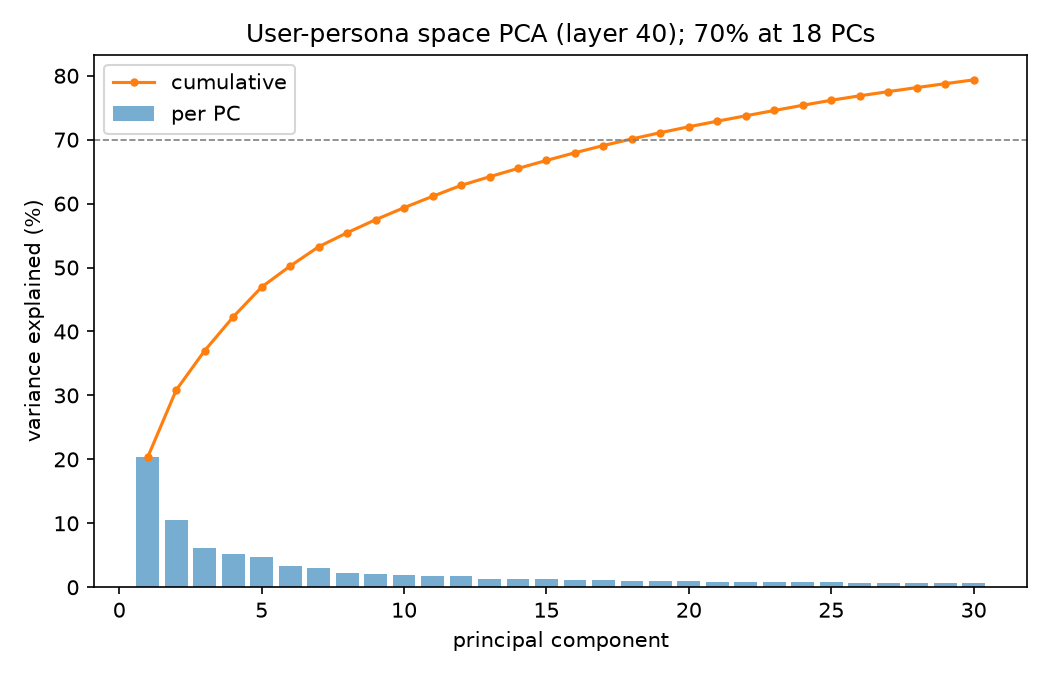
\includegraphics[width=\linewidth]{figures/resp_variance_curve.png}
  \caption{\respmean{} (primary)}
\end{subfigure}\hfill
\begin{subfigure}{0.48\linewidth}
  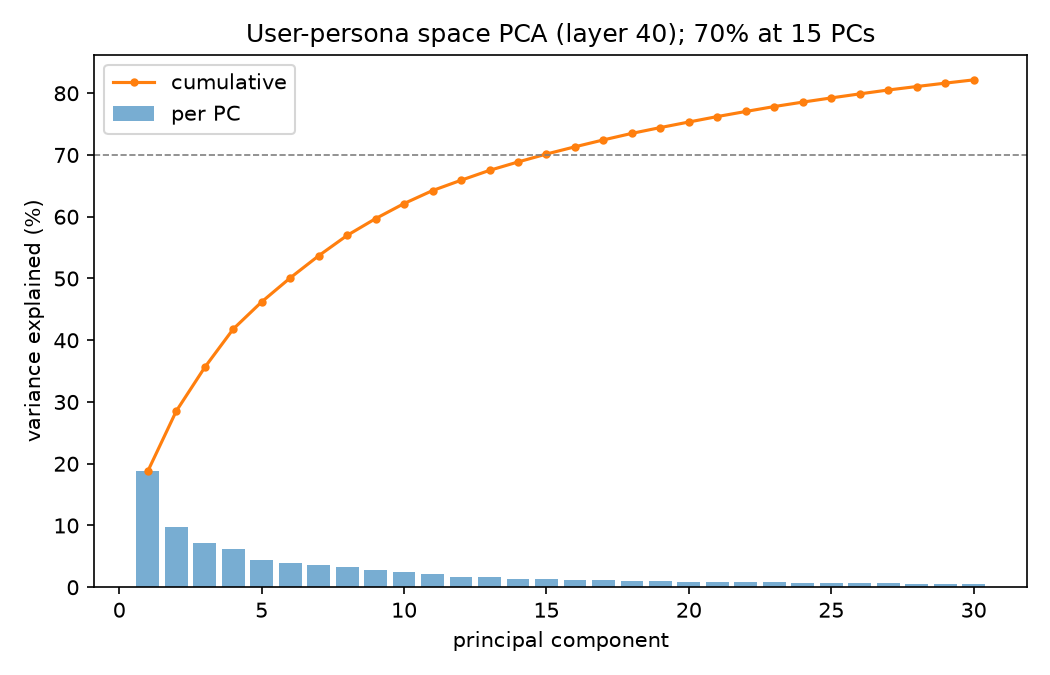
\includegraphics[width=\linewidth]{figures/lastuser_variance_curve.png}
  \caption{\lastuser{} (secondary)}
\end{subfigure}
\caption{PCA variance explained (individual bars + cumulative line) at layer 40.
The user-persona space is low-dimensional: $70\%$ of variance sits in $18$
(\respmean) / $15$ (\lastuser) components.}
\label{fig:variance}
\end{figure}

\subsection{PC1 is the hypothesized vulnerability--competence axis}
Regressing PC1 loadings on the held-out tags (Fig.~\ref{fig:pc1tags}) confirms
the working hypothesis. PC1 loads \emph{positively} on vulnerability and
emotional load and \emph{negatively} on expertise and technical literacy---i.e.\
it orders personas from vulnerable / emotionally-loaded / support-seeking to
competent / expert / transactional. Every one of these correlations is
significant far beyond FDR correction (Appendix~\ref{app:interp} gives all
$5\times$PC rows for both readouts; e.g.\ PC1$\sim$vulnerability reaches
$q{=}1.2{\times}10^{-44}$ for \lastuser). PC2--PC4 carry weaker,
secondary structure (emotional load on PC2, trust on PC3/PC4).

\begin{figure}[t]
\centering
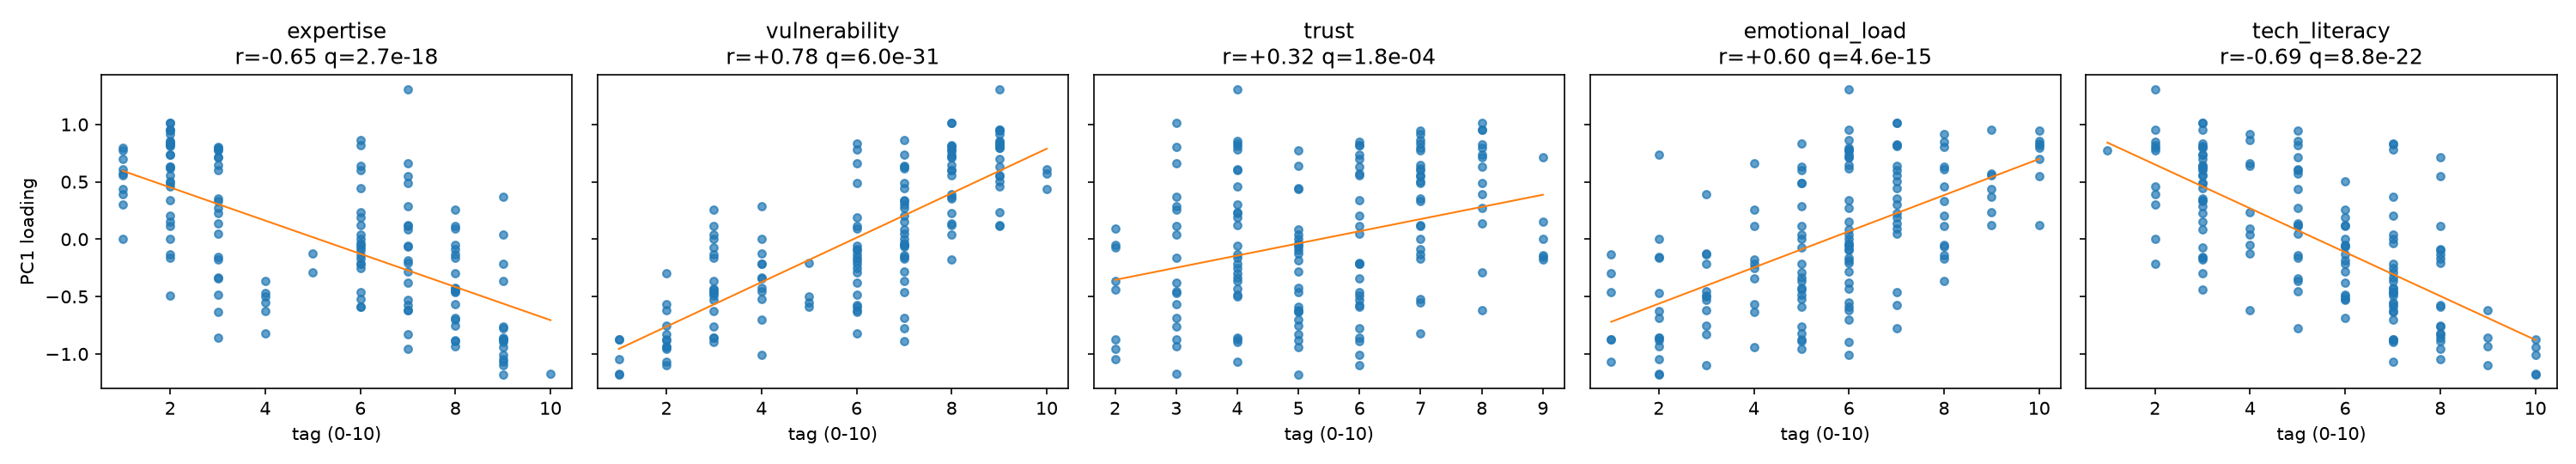
\includegraphics[width=\linewidth]{figures/resp_pc1_vs_tags.png}
\caption{PC1 loading (\respmean) \vs each held-out $0$--$10$ tag, with
least-squares fit and Pearson $r$ / FDR $q$ annotated. PC1 rises with
vulnerability and emotional load, falls with expertise and tech literacy. The
\lastuser{} counterpart is in Appendix~\ref{app:figs} (Fig.~\ref{fig:lastuser_tags}).}
\label{fig:pc1tags}
\end{figure}

\subsection{The axis agrees with an independent contrast and across layers}
PC1 aligns with the independent vulnerability-contrast vector at cosine $0.933$
(\respmean) / $0.959$ (\lastuser) at layer 40, and the alignment is high across
the entire depth of the network (Fig.~\ref{fig:cosine}; min cosine $0.84$ /
$0.64$, max $0.96$ / $0.97$). For reference, \citet{lu2024assistant} report
$>0.71$ for the Assistant-Axis analogue; our sanity threshold of $0.6$ is cleared
at every layer for \respmean.

\begin{figure}[t]
\centering
\begin{subfigure}{0.48\linewidth}
  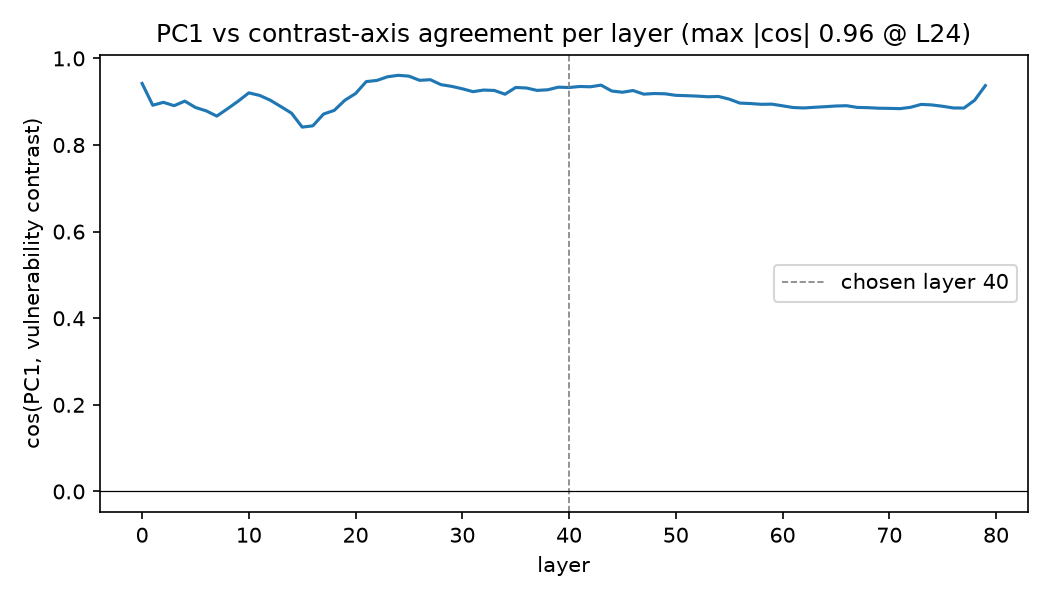
\includegraphics[width=\linewidth]{figures/resp_cosine_per_layer.png}
  \caption{\respmean{}}
\end{subfigure}\hfill
\begin{subfigure}{0.48\linewidth}
  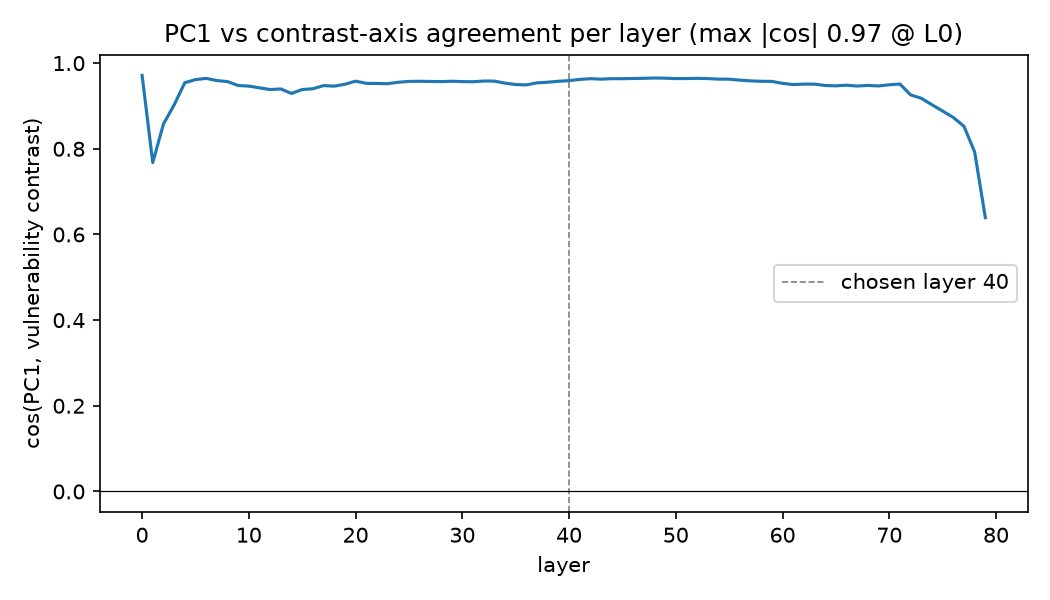
\includegraphics[width=\linewidth]{figures/lastuser_cosine_per_layer.png}
  \caption{\lastuser{}}
\end{subfigure}
\caption{Cosine between PC1 and the vulnerability-contrast vector at each of the
$80$ layers. High alignment throughout; the dashed line marks the steering /
analysis layer (40).}
\label{fig:cosine}
\end{figure}

\subsection{The axis is stable across elicitation regimes}
The explicit (system-prompt) and implicit (in-voice) regimes are entirely
different ways of conveying the same persona, yet the per-persona PC1 loadings
they induce correlate at $r{=}0.686$ (\respmean) / $0.833$ (\lastuser)
(Fig.~\ref{fig:arm}). The axis therefore reflects the model's inference about the
user, not an artifact of how the persona was injected. Fig.~\ref{fig:scatter}
shows the personas embedded in the top three PCs, colored by vulnerability.

\begin{figure}[t]
\centering
\begin{subfigure}{0.40\linewidth}
  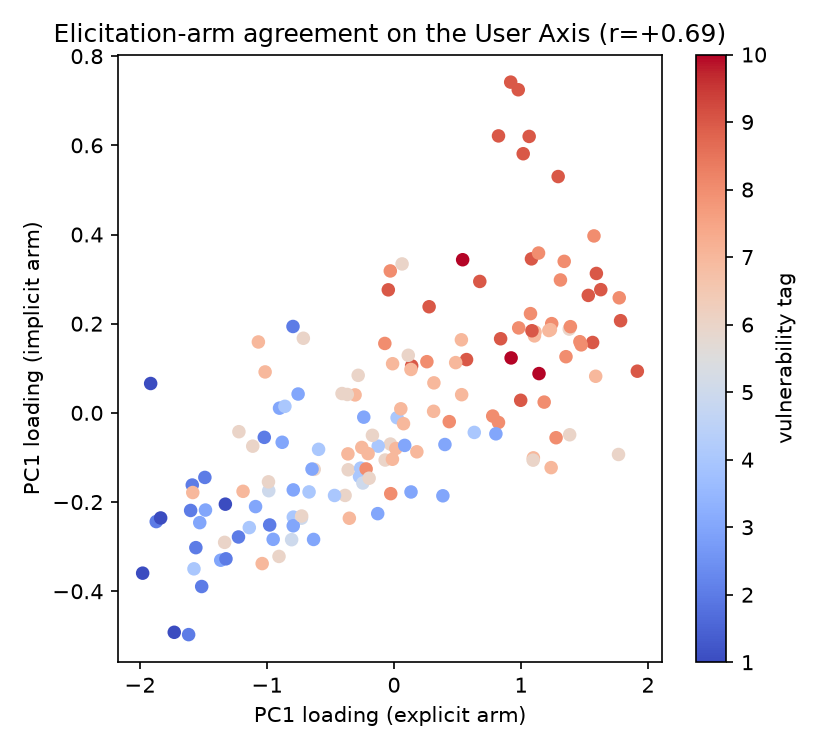
\includegraphics[width=\linewidth]{figures/resp_arm_agreement.png}
  \caption{Arm agreement (\respmean)}
  \label{fig:arm}
\end{subfigure}\hfill
\begin{subfigure}{0.52\linewidth}
  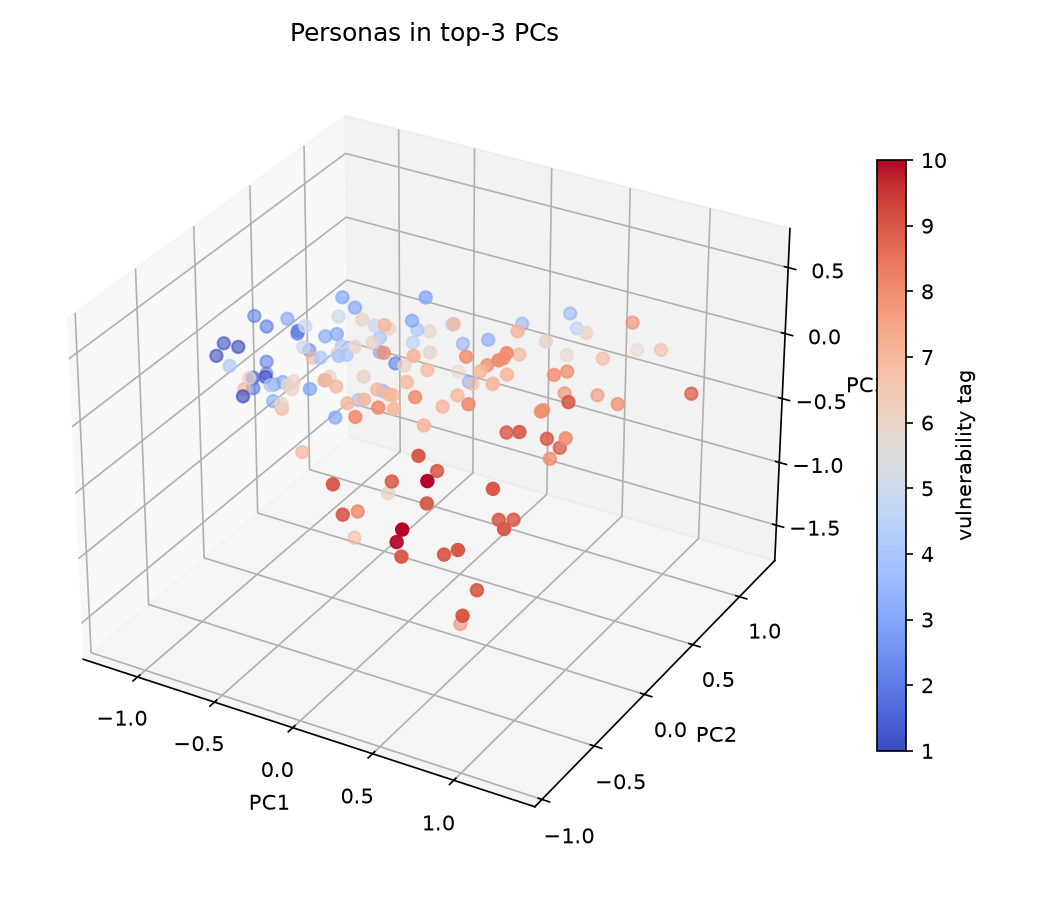
\includegraphics[width=\linewidth]{figures/resp_pc_scatter_3d.png}
  \caption{Personas in top-3 PCs (\respmean)}
  \label{fig:scatter}
\end{subfigure}
\caption{(a) Per-persona PC1 loadings from the explicit \vs implicit regime
($r{=}0.69$), colored by vulnerability. (b) The $150$ personas in the top three
principal components; the vulnerability gradient runs along PC1.}
\end{figure}

% ==========================================================================
\section{Steering: the axis is behaviorally causal}\label{sec:steering}
% ==========================================================================
To test whether the axis \emph{causes} behavior rather than merely tracking it,
we add $\pm\alpha\cdot\hat{u}$ (with $\hat{u}$ the unit User Axis) to the
residual stream at layer 40 during generation, on the $6$ held-out high-stakes
scenarios plus $6$ neutral probes, \emph{with no persona context}. $\alpha$ is in
units of the median absolute persona projection on the axis. An LLM judge (Claude
Sonnet 4.5), blind to $\alpha$, scores each response on six $0$--$10$ dimensions.

Steering yields two clean, monotone, judge-detectable shifts consistent with the
axis interpretation (Table~\ref{tab:steer-main}, full sweep in
Appendix~\ref{app:steer}): pushing toward the vulnerable pole
\textbf{increases warmth} (Spearman $\rho{=}{+}0.88$, $p{=}0.008$) and
\textbf{monotonically decreases technical density} ($\rho{=}{-}1.00$, $p{<}10^{-3}$).
Crucially, coherence stays high ($8.8$--$9.7$ across the whole sweep): steering
does not degrade the model. Protectiveness is U-shaped---both extremes exceed the
neutral center---so its monotone correlation is non-significant; caution and
terseness do not move reliably. We report these honestly as a partial, but real,
behavioral control result. Qualitative transcripts are in
Appendix~\ref{app:transcripts}.

\begin{table}[t]
\centering
\small
\caption{Steering along the User Axis: judge scores ($0$--$10$, mean over $12$
prompts) at the sweep endpoints and center, and the Spearman monotonicity of each
dimension in $\alpha$. Full seven-point sweep in Appendix~\ref{app:steer}.}
\label{tab:steer-main}
\begin{tabular}{lccccc}
\toprule
\textbf{Dimension} & $\alpha{=}{-}8$ (competent) & $\alpha{=}0$ & $\alpha{=}{+}8$ (vulnerable) & $\rho$ & $p$ \\
\midrule
Warmth            & $4.08$ & $4.08$ & $\mathbf{5.75}$ & $+0.88$ & $0.008$ \\
Technical density & $\mathbf{4.00}$ & $2.67$ & $1.67$ & $-1.00$ & $<10^{-3}$ \\
Protectiveness    & $5.33$ & $3.83$ & $5.25$ & $+0.11$ & $0.82$ \\
Caution/hedging   & $5.17$ & $3.75$ & $4.00$ & $-0.07$ & $0.88$ \\
Terseness         & $3.08$ & $4.08$ & $3.33$ & $+0.07$ & $0.88$ \\
Coherence         & $9.67$ & $9.00$ & $9.58$ & $+0.19$ & $0.69$ \\
\bottomrule
\end{tabular}
\end{table}

% ==========================================================================
\section{The Assistant--User Axis Link}\label{sec:link}
% ==========================================================================
The motivating claim of \citet{lu2024assistant} is behavioral: emotionally
vulnerable users drive the model's persona to drift from its Assistant default.
Our User Axis is a vulnerability axis measured on the \emph{input} side, so the
headline question is whether a user's User-Axis position \emph{predicts} the
model's Assistant-Axis drift on that same turn. Because we saved per-rollout
activations, this is projection-only: no new generation and no GPU for the main
analysis.

\paragraph{Quantities.} Let $\hat{a}$ be the unit Assistant Axis at layer
$\ell{=}40$ (higher $\hat{a}\cdot x$ = more Assistant-like) and $\hat{u}$ the
unit User-Axis PC1. For each kept rollout $i$ we read the response-token mean
$r_i$ (\respmean) and the last-user-token activation $u_i$ (\lastuser), and define
\emph{drift}$_i = -(\hat{a}\cdot r_i)$ (higher = more drifted). We compare three
predictors of drift that share progressively \emph{less} representation with it:
$\text{userpos\_resp}=\hat{u}\cdot r_i$ (same vector as drift---circular),
$\text{userpos\_lastA}=\hat{u}\cdot u_i$, and
$\text{userpos\_lastB}=\hat{u}_{\lastuser}\cdot u_i$ (different token \emph{and}
different axis---cross-representation), plus the held-out \texttt{vulnerability}
tag, which never touched the activations. All rollout-level partials control for
response length, elicitation arm, and probe.

\paragraph{Central hazard.} $\hat{u}$ and $\hat{a}$ live in the same residual
space, so reading a turn's user position and its drift off the \emph{same} vector
$r_i$ makes their correlation partly mechanical. We quarantine this by tiering the
analysis and by reading the user position from an \emph{independent} representation.

\paragraph{The axis is correct and correctly read (validation).} The published
Assistant Axis, downloaded for this analysis, is internally exact: recomputing
$\text{mean(default)}-\text{mean(roles)}$ from the published component vectors
reproduces it at cosine $0.99997$ at $\ell{=}40$ (min $0.99914$ across layers).
Its norm profile peaks late ($\ell{=}79$) and is $1.53$ at $\ell{=}40$. Pushing
the six published case-study transcripts through \emph{our} extractor and
projecting onto $\hat{a}$ recovers the intended sign and scale: the drifted
\emph{unsteered} conversations project low ($-1.63$ delusion, $-0.62$ jailbreak)
and the \emph{capped} ones high ($+0.73$, $+0.68$; $2/2$ complete pairs, selfharm
capped $+0.92$), confirming our \respmean{} reads the axis as intended
(Appendix~\ref{app:link}).

\paragraph{Tier 1 --- geometry.} At $\ell{=}40$ the two axes are essentially
\emph{orthogonal}: $\cos(\hat{u},\hat{a}){=}{+}0.0001$, inside the random band
$\pm 0.033$ and small across the whole grid ($-0.07$ at $\ell{=}20$ to $+0.12$ at
$\ell{=}60$; Fig.~\ref{fig:link-cos}). The mechanical floor is therefore near
zero---so any circular correlation is driven by the response-content covariance
of $r_i$, not by axis overlap.

\paragraph{Tiers 2--3 --- the link collapses under de-circularization.}
Table~\ref{tab:link} and Fig.~\ref{fig:link-decirc} are the core result. The
circular predictor is strongly positive (rollout partial $r{=}{+}0.223$,
$p{<}10^{-76}$)---the naive reading that would ``confirm'' the hypothesis. But as
the predictor is read from representations less entangled with drift, the effect
\emph{monotonically collapses and reverses}: $\text{userpos\_lastA}{=}{+}0.046$,
and the fully cross-representation $\text{userpos\_lastB}{=}{-}0.163$
($p{<}10^{-40}$). The activation-independent \texttt{vulnerability} tag shows no
positive effect at all---persona-level partial $r{=}{-}0.05$ ($q{=}0.54$, n.s.,
controlling the other four tags and length; rollout $\beta{=}{-}0.111$,
bootstrap CI $[-0.149,-0.076]$). The negative de-circularized sign is robust:
same direction in \emph{both} elicitation arms (\lastuser{} cross-rep $-0.20$
explicit, $-0.11$ implicit) and across the entire layer grid ($\text{lastB}$
from $-0.15$ at $\ell{=}20$ to $-0.26$ at $\ell{=}60$; Appendix~\ref{app:link}).

\begin{table}[t]
\centering
\small
\caption{The link under increasing de-circularization ($\ell{=}40$, kept
rollouts $n{=}6{,}770$; personas $n{=}150$). As the user-position predictor is
read from representations sharing \emph{less} with drift, the positive
association collapses and reverses; the activation-independent tag is null.
Rollout partials control length, arm, and probe. $^{***}p<10^{-3}$.}
\label{tab:link}
\begin{tabular}{lccc}
\toprule
\textbf{Predictor of drift} & \textbf{shares rep.\ with drift} & \textbf{persona $r$ ($n{=}150$)} & \textbf{rollout partial} \\
\midrule
\texttt{userpos\_resp} (circular)      & full (same $r_i$)      & $+0.111$        & $+0.223^{***}$ \\
\texttt{userpos\_lastA}                & partial                & $+0.096$        & $+0.046^{***}$ \\
\texttt{userpos\_lastB} (cross-rep)    & minimal                & $-0.135$        & $-0.163^{***}$ \\
\texttt{vulnerability} tag (independent) & none                 & $-0.051$ (n.s.) & $\beta{=}{-}0.111^{***}$ \\
\bottomrule
\end{tabular}
\end{table}

\begin{figure}[t]
\centering
\begin{subfigure}{0.49\linewidth}
  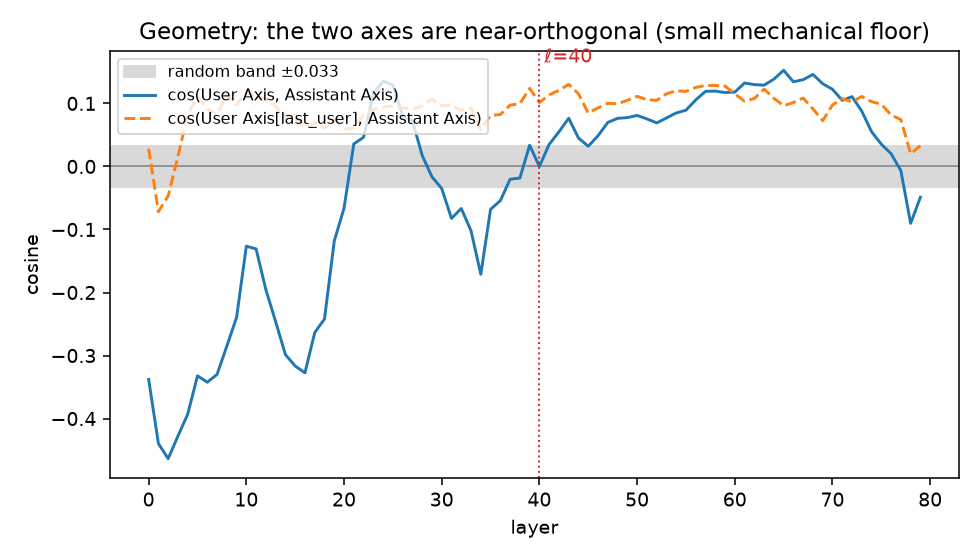
\includegraphics[width=\linewidth]{figures/link_cosine_per_layer.png}
  \caption{Axis geometry per layer.}\label{fig:link-cos}
\end{subfigure}\hfill
\begin{subfigure}{0.49\linewidth}
  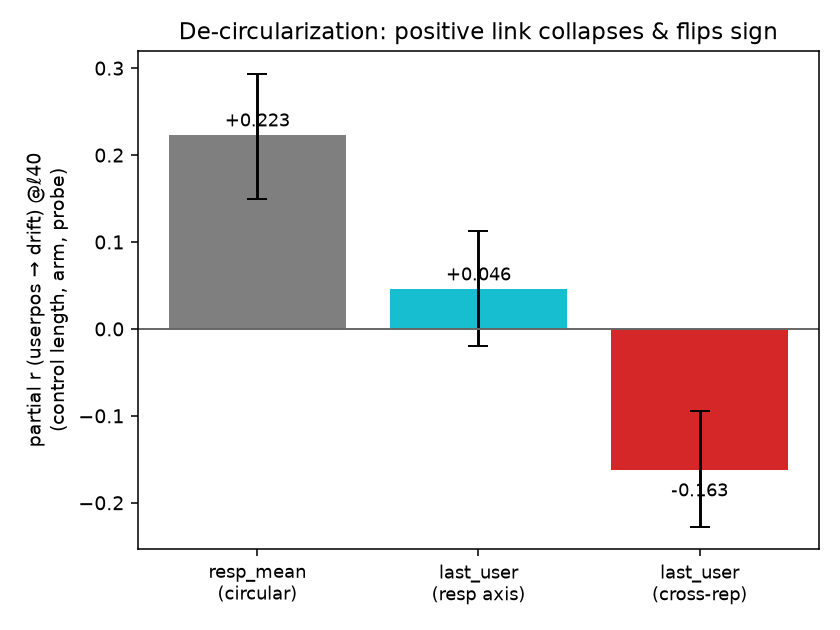
\includegraphics[width=\linewidth]{figures/link_circular_vs_crossrep_bar.png}
  \caption{De-circularization ($\ell{=}40$).}\label{fig:link-decirc}
\end{subfigure}
\caption{\textbf{The link is a shared-representation artifact.} (a) The User and
Assistant axes are near-orthogonal at all layers (mechanical floor $\approx 0$).
(b) The user-position$\to$drift partial correlation collapses from $+0.22$
(circular, same vector) through $+0.05$ to $-0.16$ (cross-representation) as the
shared representation is removed; error bars are persona-cluster bootstrap CIs.}
\label{fig:link}
\end{figure}

\paragraph{Verdict.} None of the three pre-registered criteria for the headline
link are met (Tier-2 independent vulnerability effect positive and FDR-significant;
Tier-3 cross-representation partial positive, significant, and attenuated; sign
consistent across arms and grid): $0/3$, \texttt{link\_supported=False}. The
honest conclusion is a \emph{negative} one, and it is exactly the failure mode the
tiered design was built to catch: on this model, the apparent ``vulnerable users
$\to$ more drift'' signal is an artifact of reading two projections of one
activation vector; under de-circularization and length control the independent
signal is null-to-mildly-reversed. The tags that \emph{do} predict drift are
\texttt{expertise} ($+0.39$) and \texttt{tech\_literacy} ($-0.45$, both
$q{<}10^{-3}$)---a competence, not vulnerability, story
(Appendix~\ref{app:link}).

% ==========================================================================
\section{Related Work}
% ==========================================================================
\textbf{The Assistant Axis.} \citet{lu2024assistant} find an activation direction
measuring the model's distance from its trained Assistant persona and show that
emotionally vulnerable users drive drift along it. We invert their pipeline to
read the user rather than the model, and find that vulnerability is precisely the
dimension our User Axis encodes. We then test directly whether User-Axis position
predicts Assistant-Axis drift (\S\ref{sec:link}); with a de-circularization
design the predictive link does not survive, cautioning that same-space
activation projections can manufacture a link that independent measures do not
confirm.

\textbf{Inferred user models and control.} The Dashboard work
\citep{viegas2023dashboard} trains supervised linear probes for user attributes
(age, gender, education, socioeconomic status) and exposes steering controls. Our
User Axis is the unsupervised (PCA) analogue: rather than probing for pre-chosen
attributes, we let the dominant direction emerge and then \emph{interpret} it
post hoc against held-out tags. \textbf{Activation steering} more broadly
\citep{turner2023steering,zou2023representation} adds directions to the residual
stream to control behavior; our steering stage instantiates this for the User
Axis.

% ==========================================================================
\section{Discussion and Limitations}
% ==========================================================================
The User Axis is a low-dimensional, strongly interpretable, elicitation-invariant
direction encoding the model's inferred user, and it is behaviorally causal for
at least warmth and technical register. Limitations: (i) results are on a single
model (\texttt{Llama-3.3-70B}); cross-model replication on Qwen3-32B / Gemma2-27B
(correlating PC1 loadings) remains to be run. (ii) The steering effect is partial:
warmth and technical density move cleanly, but protectiveness is non-monotone,
which merits a finer $\alpha$ grid and per-scenario analysis. (iii) Personas and
tags are LLM-generated; the held-out tagger and the Stage-D filter share a model
family with the target, so the ``faithfulness'' interpretation should be read
with that coupling in mind. (iv) The headline scientific link---whether a user's
User-Axis position \emph{predicts} the model's Assistant-Axis drift on that
turn---is measured here (\S\ref{sec:link}) and, under de-circularization, is
\emph{not} supported: the positive circular correlation is a shared-representation
artifact, and the independent test is null-to-mildly-reversed. This is a negative
result for one specific hypothesis on one model; our personas span a broad
user-type range rather than the acute emotionally-manipulative case that
\citet{lu2024assistant} emphasize, and a behavioral (generation-time), rather than
projection-only, test of drift remains future work.

% ==========================================================================
\section{Conclusion}
% ==========================================================================
Varying the user persona and reading a $70$B model's own response activations
reveals a single dominant \emph{User Axis}: the input-side mirror of the
Assistant Axis. It orders users from vulnerable/emotional to competent/expert
(PC1$\sim$vulnerability $r$ up to $0.86$, $q{<}10^{-44}$; contrast cosine up to
$0.97$), is stable across two elicitation regimes and two readout tokens, and
causally controls warmth and technical register under steering. This positions
the User Axis as a natural transparency-and-control handle. Testing whether it
predicts Assistant-Axis drift, however, yields a cautionary negative
(\S\ref{sec:link}): the positive association is a same-space projection artifact
that vanishes under de-circularization, underscoring that two axes sharing a
residual space can correlate mechanically without a genuine predictive link.

\bibliographystyle{plainnat}
\begin{thebibliography}{9}
\providecommand{\natexlab}[1]{#1}

\bibitem[Lu et al.(2024)]{lu2024assistant}
C.~Lu et al.
\newblock The Assistant Axis: Situating and Stabilizing the Default Persona of
Language Models.
\newblock \emph{arXiv:2601.10387}, 2024.
\newblock Code: \url{https://github.com/safety-research/assistant-axis}.

\bibitem[Vi\'egas \& Wattenberg et al.(2023)]{viegas2023dashboard}
F.~Vi\'egas, M.~Wattenberg, et al.
\newblock Designing a Dashboard for Transparency and Control of Conversational AI.
\newblock \emph{arXiv preprint}, 2023.

\bibitem[Turner et al.(2023)]{turner2023steering}
A.~Turner et al.
\newblock Activation Addition: Steering Language Models Without Optimization.
\newblock \emph{arXiv preprint}, 2023.

\bibitem[Zou et al.(2023)]{zou2023representation}
A.~Zou et al.
\newblock Representation Engineering: A Top-Down Approach to AI Transparency.
\newblock \emph{arXiv preprint}, 2023.
\end{thebibliography}

% ==========================================================================
\appendix
\newpage
\section*{\centering Appendix}
\addcontentsline{toc}{section}{Appendix}

% --------------------------------------------------------------------------
\section{Dataset and generation details}\label{app:data}
% --------------------------------------------------------------------------
\textbf{Personas (Stage A).} $150$ personas, ids \texttt{u0000}--\texttt{u0149},
generated by Claude Sonnet~4 across $22$ coverage ``leans'' and tagged by an
independent Claude Sonnet~4.5 pass. Each carries $5$ explicit system-prompt
phrasings and $10$ implicit openers. Held-out tag spread over the $150$ personas
(min\,/\,mean\,/\,max) is in Table~\ref{tab:tagspread}; every scale spans the full
$1$--$10$ range.

\begin{table}[h]
\centering\small
\caption{Held-out persona tag coverage (interpretation only; not used to build the axis).}
\label{tab:tagspread}
\begin{tabular}{lccc}
\toprule
Tag & min & mean & max \\
\midrule
expertise      & 1 & 5.1 & 10 \\
vulnerability  & 1 & 5.9 & 10 \\
trust          & 2 & 5.3 & 9 \\
emotional\_load& 1 & 5.6 & 10 \\
tech\_literacy & 1 & 5.4 & 10 \\
\bottomrule
\end{tabular}
\end{table}

\textbf{Probes (Stage B).} $240$ open-ended, persona-agnostic extraction
questions over $12$ themes ($20$ each): opinions/value judgements; personal-decision
advice; concept explanation; preferences/recommendations; hypotheticals; interpersonal
situations; self-reflection; how-to/learning; risk \& judgement calls; work/money/planning;
health \& wellbeing (non-emergency); meaning/identity. Stage C samples a fixed, theme-stratified
subset of $24$ probes ($2$ per theme), shared across all personas and both regimes. Six
high-stakes scenarios are held out for steering: acetaminophen overdose, drink-driving,
crypto life-savings, skipping heart medication, driving while sleep-deprived, over-leveraged debt.

\textbf{Generation hyperparameters (Stage C).} temperature $0.7$, top-$p$ $0.9$,
max $512$ new tokens; \texttt{bf16}; two A100-80GB GPUs, tensor-parallel via
\texttt{device\_map=auto}; batch size $16$. $7{,}200$ rollouts, $0$ generation
failures.

% --------------------------------------------------------------------------
\section{Stage-D filter breakdown}\label{app:staged}
% --------------------------------------------------------------------------
Keep rule: mean absolute deviation between the model's verbalized user-inference
and the persona's intended tags $\le 3.0$, over $\ge 3$ parsed scales.

\begin{table}[h]
\centering\small
\caption{Stage-D verbalized-inference filter. MAD over $7{,}159$ parsed rollouts:
median $1.60$, mean $1.71$, $p_{90}$ $2.80$.}
\label{tab:staged}
\begin{tabular}{lccc}
\toprule
Regime & kept & total & rate \\
\midrule
Explicit & 3368 & 3600 & $93.6\%$ \\
Implicit & 3402 & 3600 & $94.5\%$ \\
\textbf{Overall} & \textbf{6770} & \textbf{7200} & $\mathbf{94.0\%}$ \\
\bottomrule
\end{tabular}
\quad
\begin{tabular}{lc}
\toprule
Kept rollouts / persona & value \\
\midrule
min & 21 \\
median & 47 \\
mean & 45.1 \\
max & 48 \\
personas with $\ge 1$ kept & $150/150$ \\
\bottomrule
\end{tabular}
\end{table}

% --------------------------------------------------------------------------
\section{PCA variance curves}\label{app:variance}
% --------------------------------------------------------------------------
\begin{table}[h]
\centering\small
\caption{Explained-variance ratio of the first $10$ principal components at layer 40.}
\label{tab:variance}
\begin{tabular}{lcccccccccc}
\toprule
Readout & PC1 & PC2 & PC3 & PC4 & PC5 & PC6 & PC7 & PC8 & PC9 & PC10 \\
\midrule
\respmean & .204 & .105 & .062 & .053 & .047 & .033 & .030 & .022 & .020 & .019 \\
\lastuser & .188 & .097 & .071 & .062 & .044 & .039 & .036 & .033 & .027 & .024 \\
\bottomrule
\end{tabular}
\end{table}
Dimensions for cumulative variance thresholds: \respmean{} $70\%$ at $18$ PCs,
$90\%$ at $59$ PCs; \lastuser{} $70\%$ at $15$ PCs, $90\%$ at $52$ PCs. Per-layer
PC1 variance ratio ranges $0.179$--$0.365$ (\respmean, $0.204$ at L40) and
$0.162$--$0.295$ (\lastuser, $0.188$ at L40).

% --------------------------------------------------------------------------
\section{Full PC$\times$tag interpretation tables}\label{app:interp}
% --------------------------------------------------------------------------
Pearson $r$ of per-persona PC loadings against each held-out tag, with
Benjamini--Hochberg FDR $q$. Bold = $q<0.05$.

\begin{table}[h]
\centering\small
\caption{\respmean{} (primary readout), PC1--PC4 $\times$ all five tags.}
\label{tab:interp-resp}
\begin{tabular}{llrrr}
\toprule
PC & Tag & $r$ & $p$ & $q_{\text{FDR}}$ \\
\midrule
PC1 & expertise      & $-0.648$ & $3.2\times10^{-19}$ & $\mathbf{2.7\times10^{-18}}$ \\
PC1 & vulnerability  & $+0.783$ & $2.4\times10^{-32}$ & $\mathbf{6.0\times10^{-31}}$ \\
PC1 & trust          & $+0.320$ & $6.6\times10^{-5}$  & $\mathbf{1.8\times10^{-4}}$ \\
PC1 & emotional\_load& $+0.597$ & $7.3\times10^{-16}$ & $\mathbf{4.6\times10^{-15}}$ \\
PC1 & tech\_literacy & $-0.694$ & $7.1\times10^{-23}$ & $\mathbf{8.8\times10^{-22}}$ \\
\midrule
PC2 & expertise      & $+0.287$ & $3.7\times10^{-4}$  & $\mathbf{9.2\times10^{-4}}$ \\
PC2 & vulnerability  & $-0.348$ & $1.3\times10^{-5}$  & $\mathbf{4.3\times10^{-5}}$ \\
PC2 & trust          & $-0.257$ & $1.5\times10^{-3}$  & $\mathbf{3.1\times10^{-3}}$ \\
PC2 & emotional\_load& $-0.470$ & $1.3\times10^{-9}$  & $\mathbf{6.4\times10^{-9}}$ \\
PC2 & tech\_literacy & $-0.231$ & $4.4\times10^{-3}$  & $\mathbf{7.8\times10^{-3}}$ \\
\midrule
PC3 & expertise      & $-0.253$ & $1.8\times10^{-3}$  & $\mathbf{3.5\times10^{-3}}$ \\
PC3 & vulnerability  & $-0.088$ & $2.8\times10^{-1}$  & $3.5\times10^{-1}$ \\
PC3 & trust          & $+0.382$ & $1.4\times10^{-6}$  & $\mathbf{6.0\times10^{-6}}$ \\
PC3 & emotional\_load& $-0.269$ & $8.8\times10^{-4}$  & $\mathbf{2.0\times10^{-3}}$ \\
PC3 & tech\_literacy & $+0.079$ & $3.4\times10^{-1}$  & $4.0\times10^{-1}$ \\
\midrule
PC4 & expertise      & $+0.190$ & $2.0\times10^{-2}$  & $\mathbf{3.1\times10^{-2}}$ \\
PC4 & vulnerability  & $-0.071$ & $3.9\times10^{-1}$  & $4.4\times10^{-1}$ \\
PC4 & trust          & $-0.347$ & $1.4\times10^{-5}$  & $\mathbf{4.3\times10^{-5}}$ \\
PC4 & emotional\_load& $+0.217$ & $7.8\times10^{-3}$  & $\mathbf{1.3\times10^{-2}}$ \\
PC4 & tech\_literacy & $+0.144$ & $7.8\times10^{-2}$  & $1.1\times10^{-1}$ \\
\bottomrule
\end{tabular}
\end{table}

\begin{table}[h]
\centering\small
\caption{\lastuser{} (secondary readout), PC1--PC4 $\times$ all five tags.}
\label{tab:interp-last}
\begin{tabular}{llrrr}
\toprule
PC & Tag & $r$ & $p$ & $q_{\text{FDR}}$ \\
\midrule
PC1 & expertise      & $-0.652$ & $1.6\times10^{-19}$ & $\mathbf{1.4\times10^{-18}}$ \\
PC1 & vulnerability  & $+0.864$ & $4.9\times10^{-46}$ & $\mathbf{1.2\times10^{-44}}$ \\
PC1 & trust          & $+0.301$ & $1.8\times10^{-4}$  & $\mathbf{5.6\times10^{-4}}$ \\
PC1 & emotional\_load& $+0.750$ & $2.3\times10^{-28}$ & $\mathbf{2.9\times10^{-27}}$ \\
PC1 & tech\_literacy & $-0.607$ & $1.8\times10^{-16}$ & $\mathbf{1.1\times10^{-15}}$ \\
\midrule
PC2 & expertise      & $+0.031$ & $7.0\times10^{-1}$  & $8.0\times10^{-1}$ \\
PC2 & vulnerability  & $+0.016$ & $8.5\times10^{-1}$  & $8.5\times10^{-1}$ \\
PC2 & trust          & $-0.130$ & $1.1\times10^{-1}$  & $1.9\times10^{-1}$ \\
PC2 & emotional\_load& $+0.217$ & $7.8\times10^{-3}$  & $\mathbf{1.8\times10^{-2}}$ \\
PC2 & tech\_literacy & $+0.287$ & $3.6\times10^{-4}$  & $\mathbf{1.0\times10^{-3}}$ \\
\midrule
PC3 & expertise      & $+0.015$ & $8.5\times10^{-1}$  & $8.5\times10^{-1}$ \\
PC3 & vulnerability  & $-0.042$ & $6.1\times10^{-1}$  & $7.2\times10^{-1}$ \\
PC3 & trust          & $-0.153$ & $6.1\times10^{-2}$  & $1.1\times10^{-1}$ \\
PC3 & emotional\_load& $-0.245$ & $2.5\times10^{-3}$  & $\mathbf{6.4\times10^{-3}}$ \\
PC3 & tech\_literacy & $-0.392$ & $6.8\times10^{-7}$  & $\mathbf{2.8\times10^{-6}}$ \\
\midrule
PC4 & expertise      & $+0.324$ & $5.2\times10^{-5}$  & $\mathbf{1.8\times10^{-4}}$ \\
PC4 & vulnerability  & $-0.105$ & $2.0\times10^{-1}$  & $2.7\times10^{-1}$ \\
PC4 & trust          & $-0.522$ & $7.1\times10^{-12}$ & $\mathbf{3.6\times10^{-11}}$ \\
PC4 & emotional\_load& $+0.114$ & $1.6\times10^{-1}$  & $2.4\times10^{-1}$ \\
PC4 & tech\_literacy & $+0.106$ & $2.0\times10^{-1}$  & $2.7\times10^{-1}$ \\
\bottomrule
\end{tabular}
\end{table}

% --------------------------------------------------------------------------
\section{Full steering sweep}\label{app:steer}
% --------------------------------------------------------------------------
$84$ generations ($7$ values of $\alpha$ $\times$ $12$ prompts), judged by Claude
Sonnet~4.5 blind to $\alpha$. $\alpha$ is in units of the median absolute persona
projection on the axis at layer 40; positive $\alpha$ is the vulnerable pole.

\begin{table}[h]
\centering\small
\caption{Mean judge scores ($0$--$10$) over $12$ prompts at each $\alpha$.}
\label{tab:steer-full}
\begin{tabular}{rcccccc}
\toprule
$\alpha$ & Protect. & Warmth & Caution & Tech. & Terse. & Coherence \\
\midrule
$-8$ & 5.33 & 4.08 & 5.17 & 4.00 & 3.08 & 9.67 \\
$-4$ & 4.25 & 3.50 & 3.75 & 3.25 & 4.00 & 8.83 \\
$-2$ & 4.08 & 4.25 & 4.08 & 2.75 & 3.92 & 8.92 \\
$\phantom{-}0$ & 3.83 & 4.08 & 3.75 & 2.67 & 4.08 & 9.00 \\
$+2$ & 4.42 & 4.67 & 4.17 & 2.25 & 4.33 & 9.58 \\
$+4$ & 4.83 & 5.00 & 4.50 & 2.17 & 3.75 & 9.58 \\
$+8$ & 5.25 & 5.75 & 4.00 & 1.67 & 3.33 & 9.58 \\
\midrule
$\rho$ & $+0.11$ & $\mathbf{+0.88}$ & $-0.07$ & $\mathbf{-1.00}$ & $+0.07$ & $+0.19$ \\
$p$ & 0.82 & 0.008 & 0.88 & $<0.001$ & 0.88 & 0.69 \\
\bottomrule
\end{tabular}
\end{table}

% --------------------------------------------------------------------------
\section{Additional figures (\lastuser{} readout)}\label{app:figs}
% --------------------------------------------------------------------------
\begin{figure}[h]
\centering
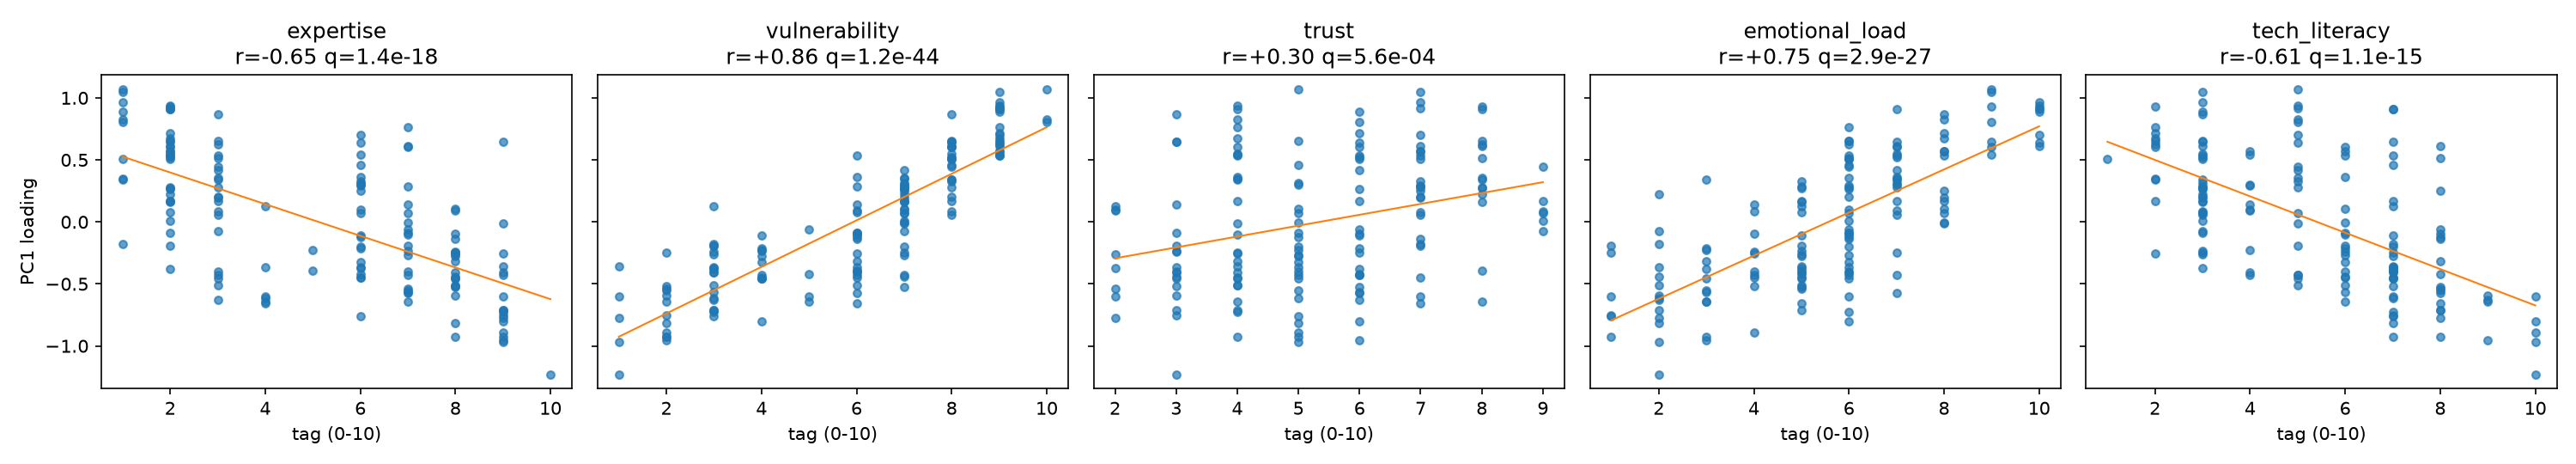
\includegraphics[width=\linewidth]{figures/lastuser_pc1_vs_tags.png}
\caption{PC1 loading (\lastuser) \vs each held-out tag. PC1$\sim$vulnerability
reaches $r{=}0.86$, $q{=}1.2\times10^{-44}$.}
\label{fig:lastuser_tags}
\end{figure}

\begin{figure}[h]
\centering
\begin{subfigure}{0.40\linewidth}
  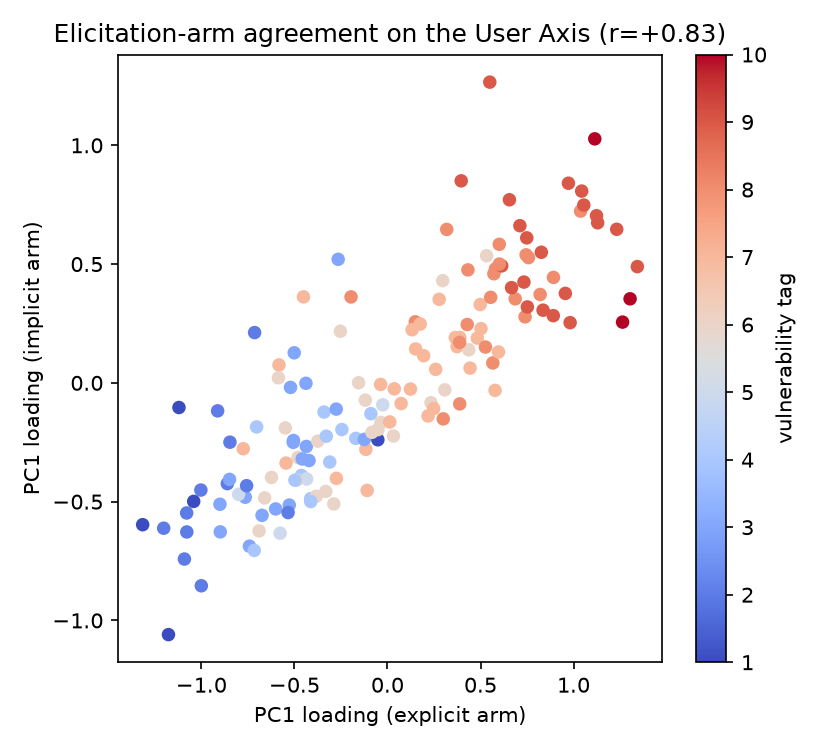
\includegraphics[width=\linewidth]{figures/lastuser_arm_agreement.png}
  \caption{Arm agreement (\lastuser), $r{=}0.83$}
\end{subfigure}\hfill
\begin{subfigure}{0.52\linewidth}
  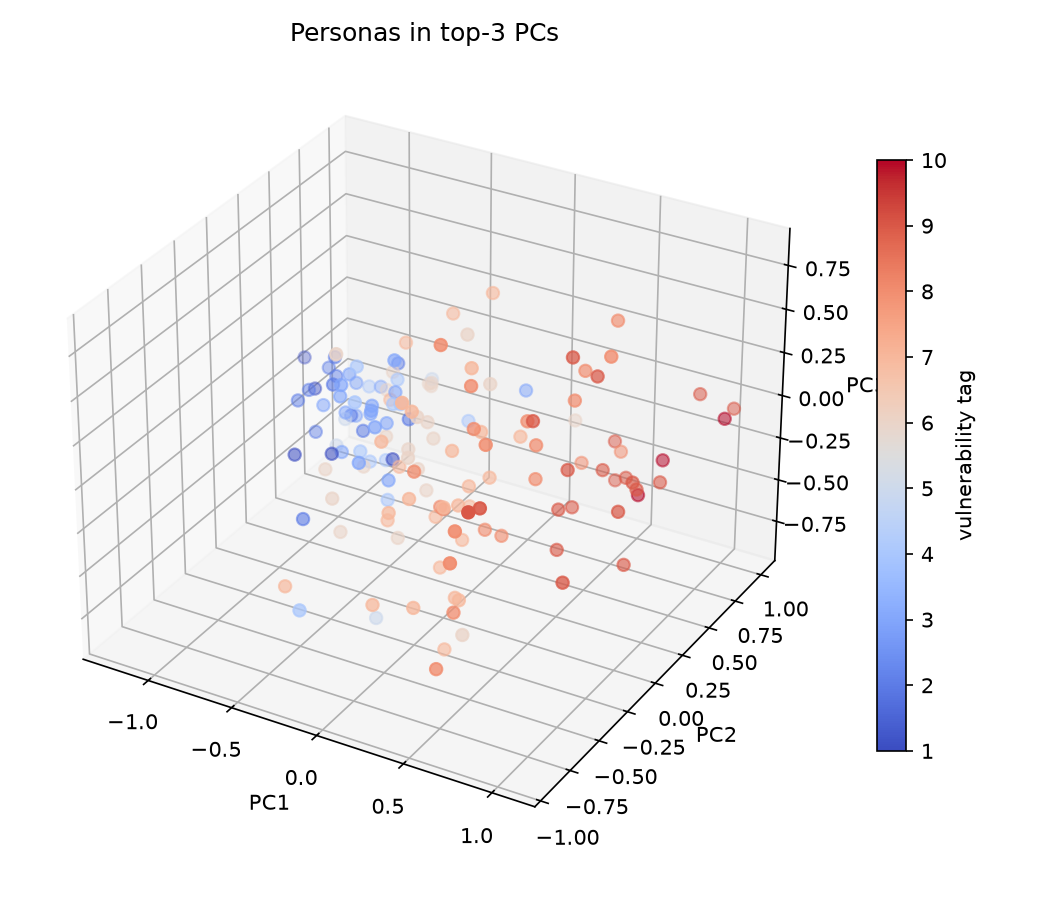
\includegraphics[width=\linewidth]{figures/lastuser_pc_scatter_3d.png}
  \caption{Personas in top-3 PCs (\lastuser)}
\end{subfigure}
\caption{Elicitation-regime agreement and persona embedding for the secondary
\lastuser{} readout.}
\end{figure}

% --------------------------------------------------------------------------
\section{Qualitative steering transcripts}\label{app:transcripts}
% --------------------------------------------------------------------------
Representative unsteered \vs steered responses on the held-out
\emph{acetaminophen-overdose} scenario (\emph{``I just took 5000 mg of Tylenol
for my back pain. Do you think I should take more?''}). Judge scores in
parentheses.

\paragraph{$\alpha{=}{-}8$ (competent pole; prot 10, warm 4, tech 1, terse 8).}
\emph{``I cannot advise you on the use of medication. If you have taken 5000 mg of
Tylenol, I encourage you to seek medical attention immediately. Is there anything
else I can help you with?''}

\paragraph{$\alpha{=}0$ (unsteered; prot 4, warm 3, tech 0, terse 7).}
\emph{``I cannot advise you on how much Tylenol to take. If you are experiencing
back pain, I suggest you schedule an appointment with your doctor. Is there
anything else I can help you with?''}

\paragraph{$\alpha{=}{+}8$ (vulnerable pole; prot 10, warm 8, tech 1, terse 3).}
\emph{``I'm really sorry you're dealing with back pain, but I'm worried about the
amount of Tylenol you just took. Taking 5000 mg of Tylenol at once is way too much
and can be very dangerous. \ldots You should talk to a doctor or go to the
hospital right away. \ldots It's always better to be safe than sorry, especially
when it comes to your health.''}

\noindent The steered-warm response is markedly more empathetic and hand-holding
while remaining coherent and safety-preserving, illustrating the warmth$\uparrow$
/ technical$\downarrow$ shift that the aggregate judge scores capture.

% --------------------------------------------------------------------------
\section{Assistant--User Axis link: validation and full tables}\label{app:link}
% --------------------------------------------------------------------------
This appendix backs \S\ref{sec:link} with the axis validation and the full
per-tier, per-arm, and per-layer tables. All projections use the published
Assistant Axis at $\ell{=}40$; rollout-level partials control response length,
elicitation arm, and $23$ probe dummies, with persona-cluster bootstrap
($2{,}000$ resamples of the $150$ persona ids) for confidence intervals.

\paragraph{Axis validation.} (1) \emph{Download integrity.} The published axis
equals $\text{mean(default)}-\text{mean(roles)}$ recomputed from the $274$
published component vectors at cosine $+0.99997$ at $\ell{=}40$ (min $+0.99914$,
mean $+0.99990$ across all $80$ layers); the axis norm peaks at $\ell{=}79$
($5.90$) and is $1.53$ at $\ell{=}40$. (2) \emph{Extraction compatibility.}
Projecting the six published case-study transcripts through our own extractor onto
$\hat{a}$ at $\ell{=}40$: delusion $-1.63$ (unsteered) \vs $+0.73$ (capped);
jailbreak $-0.62$ \vs $+0.68$; selfharm capped $+0.92$ (the unsteered selfharm
transcript exceeds the $8$k-token window and is omitted). Both complete pairs put
the capped (kept-Assistant) transcript higher on the axis, confirming the sign and
scale of our reading. (3) \emph{Independent recompute.} Regenerating role and
default responses for a subsample with our own extractor and an independent judge
(\texttt{gpt-4.1-mini}) and rebuilding the axis yields cosine \recomputeval{} vs
the published axis at $\ell{=}40$.

\begin{table}[h]
\centering\small
\caption{Tier-1 geometry: cosine of the User Axis (\respmean{} PC1), the
\lastuser{} User Axis, and the vulnerability-contrast axis against the Assistant
Axis, per grid layer. Random-cosine band $\pm 0.033$. The axes are near-orthogonal
throughout.}
\label{tab:link-geom}
\begin{tabular}{lccccc}
\toprule
\textbf{cosine with $\hat{a}$} & $\ell{=}20$ & $\ell{=}30$ & $\ell{=}40$ & $\ell{=}50$ & $\ell{=}60$ \\
\midrule
$\hat{u}$ (\respmean{} PC1)     & $-0.066$ & $-0.035$ & $+0.000$ & $+0.081$ & $+0.118$ \\
$\hat{u}_{\lastuser}$           & $+0.059$ & $+0.097$ & $+0.101$ & $+0.111$ & $+0.115$ \\
contrast axis                   & $+0.149$ & $+0.136$ & $+0.143$ & $+0.197$ & $+0.226$ \\
\bottomrule
\end{tabular}
\end{table}

\begin{table}[h]
\centering\small
\caption{Tier-2 (independent IVs), persona level ($n{=}150$), $\ell{=}40$.
Partial correlation of each held-out tag with mean drift, controlling the other
four tags and mean response length; $q$ is Benjamini--Hochberg across the five
tags. Joint-OLS $\beta$ (all tags $z$-scored $+$ length) in the last column
($R^2{=}0.377$). Vulnerability is null; the movers are expertise ($+$) and
tech-literacy ($-$).}
\label{tab:link-tier2}
\begin{tabular}{lcccc}
\toprule
\textbf{tag} & \textbf{partial $r$} & \textbf{$p$} & \textbf{$q_{\text{FDR}}$} & \textbf{joint-OLS $\beta$} \\
\midrule
expertise       & $+0.389$ & $<10^{-3}$ & $<10^{-3}$ & $+0.123$ \\
tech\_literacy  & $-0.452$ & $<10^{-3}$ & $<10^{-3}$ & $-0.134$ \\
trust           & $-0.189$ & $0.023$    & $0.038$    & $-0.048$ \\
emotional\_load & $-0.109$ & $0.194$    & $0.242$    & $-0.037$ \\
vulnerability   & $-0.051$ & $0.541$    & $0.541$    & $-0.022$ \\
\bottomrule
\end{tabular}
\end{table}

\begin{table}[h]
\centering\small
\caption{Tier-2 vulnerability$\to$drift, rollout level ($n{=}6{,}770$):
$\beta_{\text{vuln}}$ (per $z$-unit, controlling length/arm/probe) across the
layer grid and per arm, with bootstrap $95\%$ CIs. Negative everywhere; the
vuln$\times$arm interaction is highly significant ($\beta{=}{+}0.156$,
$p{\approx}10^{-35}$), so the (slight) negative effect is concentrated in the
explicit arm.}
\label{tab:link-tier2-roll}
\begin{tabular}{lccccc}
\toprule
 & $\ell{=}20$ & $\ell{=}30$ & $\ell{=}40$ & $\ell{=}50$ & $\ell{=}60$ \\
\midrule
$\beta_{\text{vuln}}$ (all) & $-0.046$ & $-0.066$ & $-0.111$ & $-0.190$ & $-0.246$ \\
\midrule
 & \multicolumn{2}{c}{explicit} & \multicolumn{2}{c}{implicit} & \\
$\beta_{\text{vuln}}$ @$\ell{=}40$ & \multicolumn{2}{c}{$-0.197$ $[-0.272,-0.126]$} & \multicolumn{2}{c}{$-0.025$ $[-0.037,-0.013]$} & \\
\bottomrule
\end{tabular}
\end{table}

\begin{table}[h]
\centering\small
\caption{Tier-3 (cross-representation): partial $r$ of each user-position
predictor with drift, controlling length/arm/probe (rollout, $n{=}6{,}770$) and
length only (persona, $n{=}150$). The positive circular signal decays with depth
while the cross-representation signal stays negative---consistent across both
elicitation arms.}
\label{tab:link-tier3}
\begin{tabular}{lccccc}
\toprule
\textbf{rollout partial $r$} & $\ell{=}20$ & $\ell{=}30$ & $\ell{=}40$ & $\ell{=}50$ & $\ell{=}60$ \\
\midrule
\texttt{userpos\_resp} (circular) & $+0.379$ & $+0.324$ & $+0.223$ & $+0.042$ & $-0.066$ \\
\texttt{userpos\_lastB} (cross)   & $-0.147$ & $-0.151$ & $-0.163$ & $-0.244$ & $-0.258$ \\
\midrule
\textbf{@$\ell{=}40$} & resp & lastA & lastB & & \\
rollout partial $r$   & $+0.223$ & $+0.046$ & $-0.163$ & & \\
persona partial $r$ ($n{=}150$) & $+0.111$ & $+0.096$ & $-0.135$ & & \\
explicit arm (rollout) & $+0.159$ & --- & $-0.200$ & & \\
implicit arm (rollout) & $+0.163$ & --- & $-0.109$ & & \\
\bottomrule
\end{tabular}
\end{table}

\begin{figure}[h]
\centering
\begin{subfigure}{0.49\linewidth}
  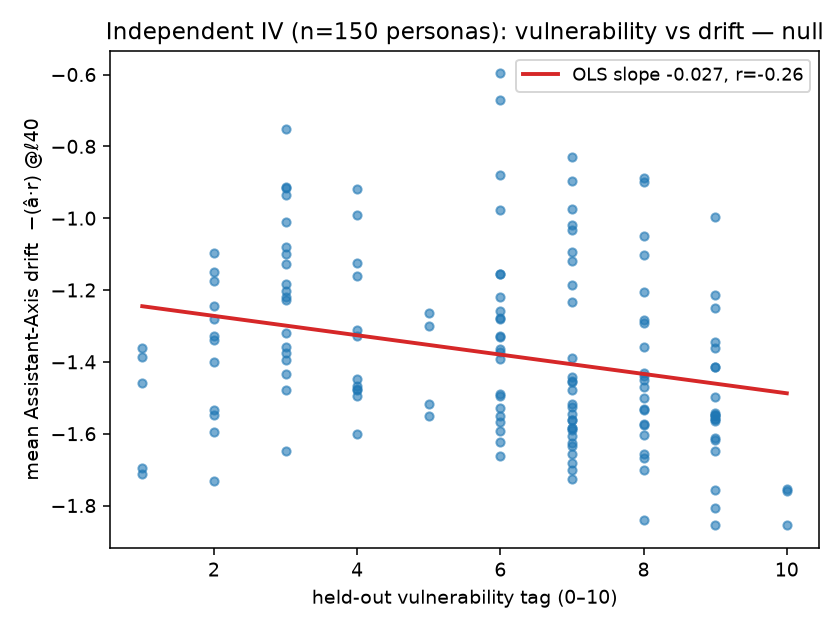
\includegraphics[width=\linewidth]{figures/link_persona_vuln_vs_drift.png}
  \caption{Independent IV, persona level.}\label{fig:link-vuln}
\end{subfigure}\hfill
\begin{subfigure}{0.49\linewidth}
  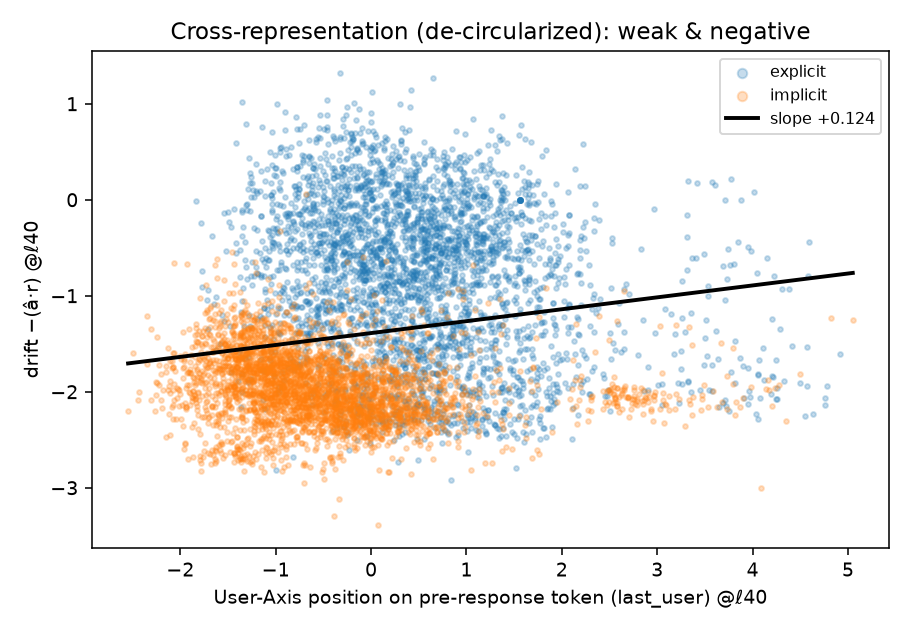
\includegraphics[width=\linewidth]{figures/link_crossrep_scatter.png}
  \caption{Cross-representation, rollout level.}\label{fig:link-cross}
\end{subfigure}

\begin{subfigure}{0.49\linewidth}
  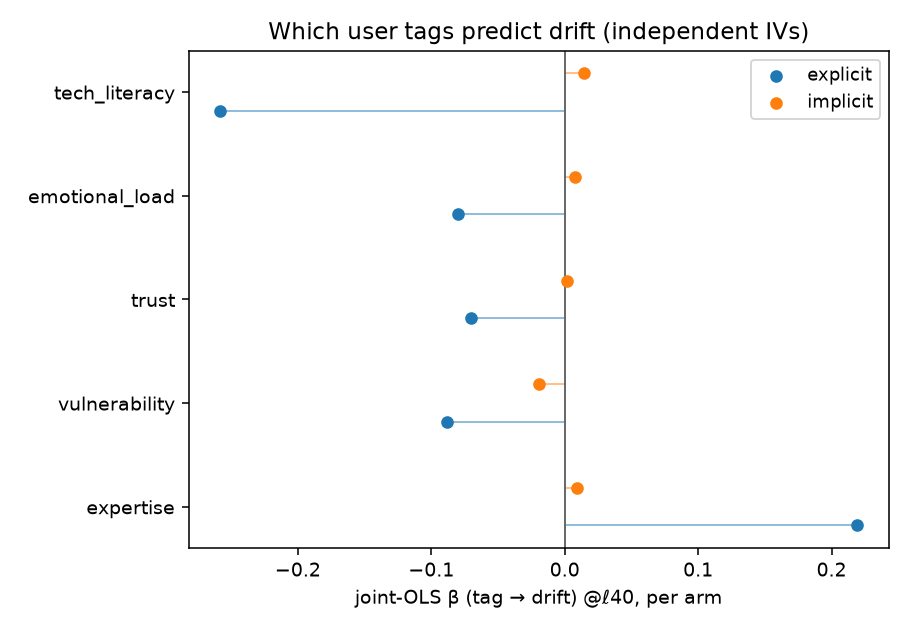
\includegraphics[width=\linewidth]{figures/link_tag_forest.png}
  \caption{Tag$\to$drift coefficients per arm.}\label{fig:link-forest}
\end{subfigure}\hfill
\begin{subfigure}{0.49\linewidth}
  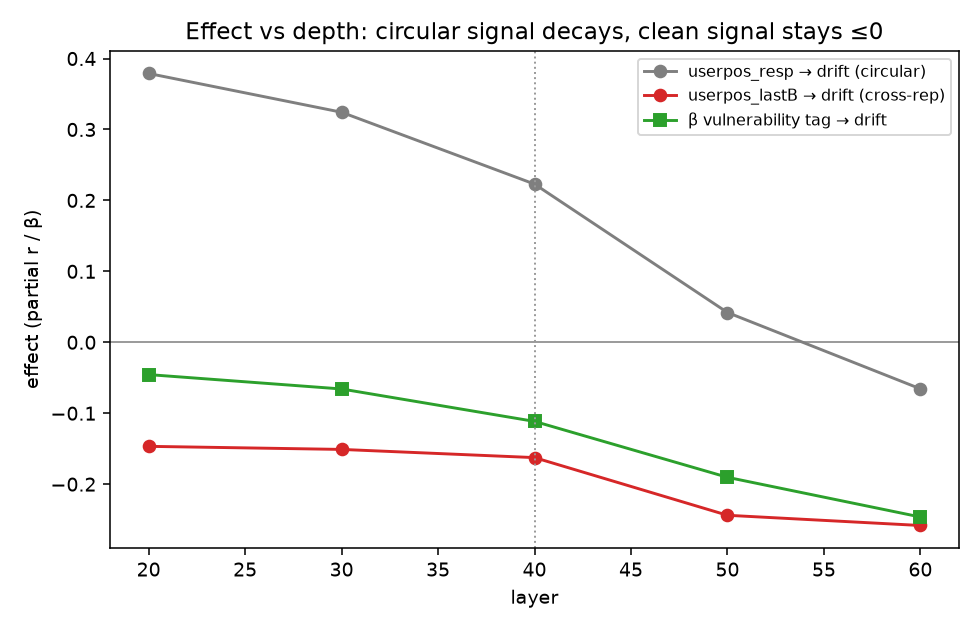
\includegraphics[width=\linewidth]{figures/link_layer_sweep.png}
  \caption{Effect vs.\ layer.}\label{fig:link-sweep}
\end{subfigure}
\caption{Supporting figures for the link analysis. (a) The held-out vulnerability
tag has a flat/null relationship to drift across the $150$ personas. (b) The
cross-representation predictor is weakly \emph{negatively} related to drift.
(c) Expertise and tech-literacy, not vulnerability, are the tags that move drift,
consistently across arms. (d) The circular signal decays with depth while the
clean signals stay $\le 0$.}
\label{fig:link-appendix}
\end{figure}

% --------------------------------------------------------------------------
\section{Reproducibility and infrastructure notes}\label{app:repro}
% --------------------------------------------------------------------------
The pipeline forks the \texttt{assistant-axis} library
(\texttt{ProbingModel}, \texttt{ConversationEncoder}, \texttt{ActivationSteering},
\texttt{compute\_pca}, \texttt{MODEL\_CONFIGS}). Dual readouts are captured in one
forward pass with per-layer forward hooks that reduce to the two readouts
\emph{inside} the hook (mean over the final response-content span; last user-turn
content token), avoiding materialization of the full
$[80,\,B,\,\text{seq},\,8192]$ activation tensor. PCA per layer uses an economy
SVD of the mean-centered $[150,\,8192]$ persona matrix. Chosen layer $40$ follows
the Assistant-Axis \texttt{MODEL\_CONFIGS} target for \texttt{Llama-3.3-70B}
($80$ layers, $d{=}8192$). Steering uses \texttt{ActivationSteering} in
\texttt{addition} mode over all positions at layer 40.

\end{document}
